%   Filename    : chapter_1.tex 
\chapter{Introduction}
\label{sec:researchdesc}    %labels help you reference sections of your document

\section{Overview of the Current State of Technology}
\label{sec:overview}
The Department of Environment and Natural Resources (DENR) expressed in their website that monitoring air quality is essential in reducing air pollution and they plan to protect the environment and public health by strengthening their air quality monitoring systems \cite{DENR2020}.

An example of air quality monitoring system that the DENR uses is the Differential Optical Absorption Spectroscopy (DOAS). \cite{DENR_ND}. DOAS captures light that passes through the atmosphere, to measure different wavelengths that were absorbed by different gasses. This method can accurately measure trace gasses absorption and it is simpler and less expensive to operate. DOAS, however, is greatly affected by turbulence in the atmosphere \cite{PlattEtAl2008}. DENR also has particulate matter stations that records PM 2.5 and PM 10. \cite{DENR_ND}

DOAS equipment needs frequent maintenance to be able to operate normally. In a news report by \cite{enano_subingsubing_2019} regarding air pollution at EDSA it was stated that the maintenance of these equipment requires “hundreds of thousands of pesos”.

Currently, The way to access the data from the AQMS stations is through the website (https://air.emb.gov.ph/ambient-air-quality-monitoring/) and the play store application. Figure \ref{fig:PAQIApp} shows the contents of the application.\\

  
%--- the following example shows how to include a figure in PNG format
\begin{figure}[t]                %-- use [t] to place figure at top, [b] to place at the bottom, [h] for here
   \centering                    %-- use this to center the figure
   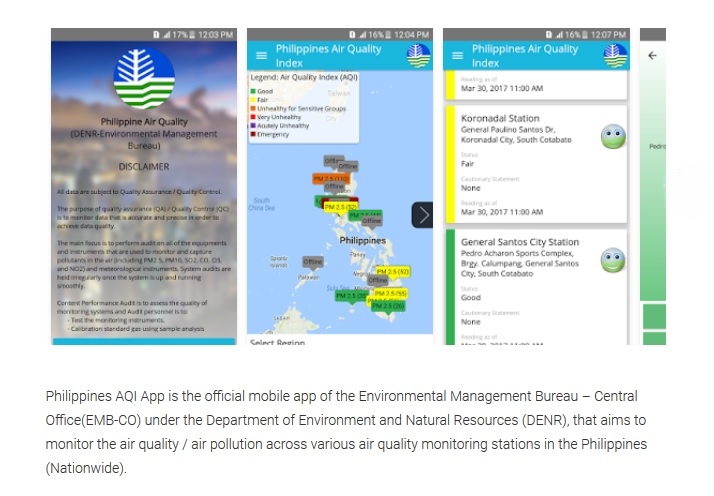
\includegraphics[width=120mm,scale=1.5]{PAQIApp.jpg}      %-- include image file named as "disneychart.png" 
   \caption{Screen capture of the mobile application of the Philippines Air Quality Index. Photo taken from https://air.emb.gov.ph/ambient-air-quality-monitoring/ 
}
    \label{fig:PAQIApp}
\end{figure}


In the mobile application disclaimer it is stated that the system audits are irregular and all data are subject to quality Assurance and quality control. This means that the end user may not get the accurate data that they expect when using the application. Moreover, monitoring stations are not online 24/7 which makes the data less accessible.


\section{Problem Statement}
	Air pollution has become a global problem over the years. As stated by \cite{Akimoto2004}, the availability of the CO2 concentrations on the Measurement of Air Pollution from Satellite (MAPS) instrument in 1981 shows high concentrations of the greenhouse gas over tropical Asia, Africa, and South America. Not only does this date provide evidence that this has become an international issue, it also shows how fossil fuel combustion can have an impact on air quality. 

The Philippines, a country located in tropical Asia, is not devoid of these issues. An article by \cite{abano_2019} states that a 2018 study by the World Health Organization reports the Philippines has ranked third among the countries with air pollution related deaths. These deaths are tied to harmful particles entering a person’s lungs, which can lead to multiple different ailments and diseases such as: heart disease, lung cancer, and respiratory infections, to name a few.

Air pollution can come from different sources, whether it be from stationary constructs like factories or mobile sources such as cars. \cite{EMB_2015}  An air quality status report by the Department of Environment and Natural Resources (2015) shows that 65\% of the air pollutants come from these mobile sources. This worsened as the EMB’s official site \cite{EMB_2018} states that based on the Emissions Inventory of 2018, the pollutant contribution of mobile sources has increased to  74\%. In places where traffic is congested could be a huge contributing factor to vehicular emissions. \cite{vergel_yai2000} states that the congestion in the roads of Metro Manila contributes to the worsening air quality, especially in the vicinity of the road environment.

In the country’s attempt to mitigate the atmospheric issues, the Philippine Clean Air Act of 1999 (Republic Act No. 8749) was passed. \cite{FAO} It entails the resolution of creating a national program of air pollution management, mainly focusing on pollution prevention. Two decades later and the country still sees increasing pollutants in the air and does not show signs of the improvement that was planned.

In addition to creating air pollution management programs, the Philippine Clean Air Act also aimed to utilize mass media communication in order to create awareness and active participation in air quality planning and monitoring. Considering that the available technology dedicated to monitoring the air quality in the country is sparsely spread throughout the country, being accessible to more citizens can help in creating awareness at a lower cost. With the aforementioned said, a system that could satisfy that goal can be created with the newer technologies that were not present in the decades prior. Thus, Hazy was constructed, a system that can gather information from vehicles – one of the biggest contributors of air pollution and provide an estimate to emissions produced, as a solution to these problems. 


\section{Research Objectives}
\label{sec:researchobjectives}

\subsection{General Objective}
\label{sec:generalobjective}


The general objective of the study is to develop an application that calculates the location’s average amount of  fine particulate matter ($PM_{2.5}$) emission from vehicles through the use of a vehicle detection system. This system will identify the vehicles on the street from a live camera feed. The system will integrate the values of $PM_{2.5}$  of different vehicles, which will be utilized to assign values to on-screen vehicles for their total average to be calculated. The average $PM_{2.5}$ value will then be displayed on the screen for the user to see.



\subsection{Specific Objectives}
\label{sec:specificobjectives}

%
%  \begin{comment} ... \end{comment} is used for multiple lines of comment
%
This study specifically aims to:


\begin{comment}
% IPR acknowledgement: the following sentences and examples are from Ethel Ong's slides 
%     on Research Objectives
How to formulate your research objectives:
1. Identify what research steps do you need to perform to achieve your general objective.
2. Identify the questions that must be answered for you to achieve your general objective.
    Thereafter, convert these questions into action statements

Example #1:

Research Question:
  What are the general features of a web-based learning environment?

Specific Objective:
   To review existing web-based learning environment that teaches language learning for children


Example #2:

Research Question:
   How will you represent commonsense knowledge for use by computer systems?

Specific Objective:
   To identify knowledge representation approaches used by existing story generation systems

Example #3:
Research Question:
   What types of storytelling knowledge are needed to generate stories?

Specific Objective:
    To identify the different types of storytelling knowledge used in generating stories

Example #4:
Research Question:
    What machine learning approaches will you utilize?

Specific Objective:
    To determine existing machine learning algorithms [that can be used in training the computer system to detect cyberbullying cases] 

Example #5: Research Question:
    How will your research output be evaluated?

Specific Objective:
    To define evaluation metrics for validating the accuracy of the translation

\end{comment}

%
%  The following are example specific objectives; replace them with your own 
%

\begin{enumerate}
   
   \item To study YOLOv5 and its components to develop the application
   \item To implement real-time vehicle detection and counting into a system that can be used on a live camera feed
   \item To gather a collection of images of vehicles to be used for training for a system to detect real-time traffic footage to calculate the overall emission of an area based on the vehicles' average $PM_{2.5}$ emission.

\end{enumerate}


\section{Scope and Limitations of the Research}
\label{sec:scopelimitations}
This application mainly focused on the PM2.5 emitted by traffic in the Philippines, where the researchers reside as of writing the paper. Thus, it will only be set up and used on the vehicles that travel within the country. For this reason, this project has some significant difficulties in using existing databases of vehicles that are mainly found locally (i.e. jeepneys and tricycles), with little to no readily available databases existing to be utilized in the study. To avoid said vehicles from not being detected, the researchers opted to take pictures and videos of the vehicles in traffic to be used as training data. These vehicles were recorded on a smartphone and were uploaded in Roboflow, which was used to annotate them as their respective vehicle type. 

However, since the vehicles with no existing databases are taken and curated by the researchers within a small time frame, this could lead to inaccuracies as the frequency of a specific vehicle to appear on the road when recording is not guaranteed. Thus, lacking in representation compared to other common vehicles such as cars.

Furthermore, this study will be utilizing the YOLOv5 object identification framework  and is thus limited to the features of that version. Any other features and upgrades that are present in future versions of the framework will not be included in the study. 



\begin{comment}

%
% IPR acknowledgement: the sentences inside this comment are from Ethel Ong's slides on Scope and Limitations of the Research
%
Generally, one paragraph should be allotted for each of your research objectives.

Each paragraph contains a brief overview of the concept/theory and the purpose of doing the associated objective.

Each paragraph also includes a description of the scope/limitation of your study.

* Please refer to the slides for examples.

\end{comment}


\section{Significance of the Research}
\label{sec:significance}

The main objective of this study is to create an application that helps its users identify the $PM_{2.5}$ levels of a traffic congested area through a live video feed over the road. It serves as an example on how computer vision can be utilized to get an estimate of the pollutants in an area via tracking the vehicles they come from. This poses benefits to users that want to acquire information on the pollutant levels in traffic congested areas. Civilians such as joggers can plan their travel accordingly to avoid areas if $PM_{2.5}$ levels get too high.

For the environment sector, this study can help contribute to the air pollution awareness in the country, in which such data can be utilized when creating future plans and protocols to combat the rising concern for the country’s air quality. The system is also open source so it is a benefit for the general public to use without needing a full set of gear to check on pollution levels.

Lastly, as interest in the computer vision field of vehicle identification and recognition systems increases, this study can contribute to future research on said field. The study can be of help to future researchers on the topics of: computer vision and tracking vehicular greenhouse gasses emissions. This may also provide data to vehicle image databases through the contribution of local vehicles from the Philippines.




\begin{comment}
If applicable, describe possible commercialization and/or innovation in your research.
\end{comment}


